
%----------------------------------------------------------------------------------------
%	PACKAGES AND OTHER DOCUMENT CONFIGURATIONS
%----------------------------------------------------------------------------------------

\documentclass[
11pt,
oneside, 
english,
singlespacing,
headsepline, 
fleqn
]{MastersDoctoralThesis} 

\usepackage[utf8]{inputenc} 
\usepackage[T1]{fontenc} 
\usepackage{amsmath} 
\usepackage{palatino} 
\usepackage[backend=bibtex,style=authoryear,maxcitenames=2, natbib=true]{biblatex} 
\addbibresource{example.bib} 
\setlength{\parindent}{0pt} 
\usepackage{listings}
\usepackage{color}
\usepackage{gensymb}
\lstset{frame=tb,
  language=Python,
  aboveskip=3mm,
  belowskip=3mm,
  showstringspaces=false,
  columns=flexible,
  basicstyle={\small\ttfamily},
  numbers=none,
  numberstyle=\tiny\color{black},
  keywordstyle=\color{cyan},
  commentstyle=\color{red},
  stringstyle=\color{green},
  breaklines=true,
  breakatwhitespace=true,
  tabsize=3
}
\usepackage{longtable}
\usepackage{textcomp}


%----------------------------------------------------------------------------------------
%	MARGIN SETTINGS
%----------------------------------------------------------------------------------------

\geometry{
	paper=a4paper, % Change to letterpaper for US letter
	inner=2.5cm, % Inner margin
	outer=2.5cm, % Outer margin
	bindingoffset=.5cm, % Binding offset
	top=1.5cm, % Top margin
	bottom=1.5cm, % Bottom margin
	%showframe, % Uncomment to show how the type block is set on the page
}

%----------------------------------------------------------------------------------------
%	THESIS INFORMATION
%----------------------------------------------------------------------------------------

\thesistitle{An Exploration of Alternative Features in Micro-Finance Loan Default Prediction Models} % Your thesis title, this is used in the title and abstract, print it elsewhere with \ttitle
\supervisor{Mr S \textsc{Britz}} % Your supervisor's name, this is used in the title page, print it elsewhere with \supname
\examiner{} % Your examiner's name, this is not currently used anywhere in the template, print it elsewhere with \examname
\degree{Masters of Science in Data Science} % Your degree name, this is used in the title page and abstract, print it elsewhere with \degreename
\author{Devon \textsc{Stone}} % Your name, this is used in the title page and abstract, print it elsewhere with \authorname

\university{\href{https://www.uct.ac.za/}{University of Cape Town}} % Your university's name and URL, this is used in the title page and abstract, print it elsewhere with \univname
\faculty{\href{http://www.stats.uct.ac.za}{Department of Statistical Sciences}} % Your faculty's name and URL, this is used in the title page and abstract, print it elsewhere with \facname
\AtBeginDocument{
\hypersetup{pdftitle=\ttitle} % Set the PDF's title to your title
\hypersetup{pdfauthor=\authorname} % Set the PDF's author to your name
\hypersetup{pdfkeywords=\keywordnames} % Set the PDF's keywords to your keywords
}

\begin{document}
\frontmatter % Use roman page numbering style (i, ii, iii, iv...) for the pre-content pages
\pagestyle{plain} % Default to the plain heading style until the thesis style is called for the body content

%----------------------------------------------------------------------------------------
%	TITLE PAGE
%----------------------------------------------------------------------------------------

\begin{titlepage}
\begin{center}

\vspace*{.06\textheight}
{\scshape\huge \univname\par}\vspace{1cm} % University name\

\includegraphics[width=0.45\textwidth]{images/logo.png}\\[0.6cm] % University/department logo
\HRule \\[0.4cm] % Horizontal line
{\huge \bfseries \ttitle\par}\vspace{0.4cm} % Thesis title
\HRule \\[1cm] % Horizontal line
 
\begin{minipage}[t]{0.4\textwidth}
\begin{flushleft} \large
\emph{Author:}\\
\href{https://devon12stone.github.io/E-Portfolio2/}{\authorname} % Author name - remove the \href bracket to remove the link
\end{flushleft}
\end{minipage}
\begin{minipage}[t]{0.4\textwidth}
\begin{flushright} \large
\emph{Supervisor:} \\
\href{http://www.jamessmith.com}{\supname} % Supervisor name - remove the \href bracket to remove the link  
\end{flushright}
\end{minipage}\\
\vspace{2cm}
\large \textit{A thesis submitted in the partial fulfilment for a \degreename}\\[0.3cm] % University requirement text
\textit{from the}\\[1cm]
{\scshape\LARGE\facname\par}\vspace{1cm} % faculty name\
{\large \today}\\[2cm] % Date
\vfill
\end{center}
\end{titlepage}

%----------------------------------------------------------------------------------------
%	DECLARATION PAGE
%----------------------------------------------------------------------------------------

\begin{declaration}
\addchaptertocentry{\authorshipname} % Add the declaration to the table of contents
\noindent I, \authorname, declare that this thesis titled, \enquote{\ttitle} and the work presented in it are my own. I confirm that I know the meaning of plagiarism and declare that all the work in the document, save for that which is properly acknowledged, is my own. This dissertation has been submitted to the Turnitin module (or  equivalent similarity and originality checking software) and I confirm that my supervisor has seen my report and any concerns revealed by such have been resolved with my supervisor. \\
 
\noindent Signed:\\
\rule[0.5em]{25em}{0.5pt} % This prints a line for the signature
 
\noindent Date:\\
\rule[0.5em]{25em}{0.5pt} % This prints a line to write the date
\end{declaration}

\cleardoublepage

%----------------------------------------------------------------------------------------

%	ABSTRACT PAGE
%----------------------------------------------------------------------------------------

\begin{abstract}
\addchaptertocentry{\abstractname} % Add the abstract to the table of %contents

Despite recent developments financial inclusion remains a large issue for the World's unbanked population. Financial institutions - both larger corporations and micro-finance companies - have begun to provide solutions for financial inclusion. The solutions are delivered using a combination of machine learning and alternative data. \\

This minor dissertation focuses on investigating whether alternative features generated from Short Messaging Service (SMS) data and Android application data contained on borrowers' devices can be used to improve the performance of loan default prediction models. The improvement gained by using alternative features is measured by comparing loan default prediction models trained using only traditional credit scoring data to models developed using a combination of traditional and alternative features. Furthermore, the paper investigates which of 4 machine learning techniques is best suited for loan default prediction. The 4 techniques investigated are logistic regression, random forests, extreme gradient boosting, and neural networks. Finally the paper identifies whether or not accurate loan default prediction models can be trained using only the alternative features developed throughout this minor dissertation. \\

The results of the research show that alternative features improve the performance of loan default prediction across 5 performance indicators, namely overall prediction accuracy, repaid prediction accuracy, default prediction accuracy, F1 score, and AUC. Furthermore, extreme gradient boosting is identified as the most appropriate technique for loan default prediction. Finally, the research identifies that models trained using the alternative features developed throughout this project can accurately predict loan that have been repaid, the models do not accurately predict loans that have not been repaid.   


\end{abstract}

%----------------------------------------------------------------------------------------
%	ACKNOWLEDGEMENTS
%----------------------------------------------------------------------------------------

\begin{acknowledgements}
\addchaptertocentry{\acknowledgementname} % Add the acknowledgements to the table of contents
My deepest thanks are extended to my supervisor, Mr Stefan Britz, for his guidance and insights throughout this project. I would like to thank my family for their constant support. Finally, to my friend James Leslie, thank you for your input and support throughout the project.  
\end{acknowledgements}

%----------------------------------------------------------------------------------------
%	LIST OF CONTENTS/FIGURES/TABLES PAGES
%----------------------------------------------------------------------------------------

\tableofcontents % Prints the main table of contents

\listoffigures % Prints the list of figures
\addchaptertocentry{List of Figures} % Add the list of figures to the table of contents

\listoftables % Prints the list of tables
\addchaptertocentry{List of Tables} % Add the list of tables to the table of contents


%----------------------------------------------------------------------------------------
%	ABBREVIATIONS
%----------------------------------------------------------------------------------------

\begin{abbreviations}{ll} % Include a list of abbreviations (a table of two columns)
\addchaptertocentry{List of Abbreviations} % Add the list of abbreviations to the table of contents
\textbf{SMS} & \textbf{S}hort \textbf{M}essaging \textbf{S}ervice\\
\textbf{LDA} & \textbf{L}inear \textbf{D}iscriminant \textbf{A}anlysis\\
\textbf{CART} & \textbf{C}lassification and \textbf{R}egression \textbf{T}rees\\
\textbf{NN} & \textbf{N}erual  \textbf{N}etwork\\
\textbf{SVM} & \textbf{S}upport  \textbf{V}ector \textbf{M}achine \\
\textbf{ROC} & \textbf{R}eceiver  \textbf{O}perating \textbf{C}haracteristic \\
\textbf{AUC} & \textbf{A}rea  \textbf{U}nder \textbf{C}urve \\
\textbf{SMOTE} & \textbf{S}ynthetic \textbf{M}inority \textbf{O}ver-\textbf{S}ampling \textbf{T}echnique\\
\textbf{MFIs} & \textbf{M}icro \textbf{F}inance \textbf{I}nstitutions\\
\textbf{SVD} & \textbf{S}ingle \textbf{V}alue \textbf{D}ecomposition\\
\textbf{KNN} & \textbf{K}- \textbf{N}earest \textbf{N}eighbours\\
\textbf{REF} & \textbf{R}ecursive \textbf{F}eature \textbf{E}limination\\
\textbf{XGBoost} & \textbf{X}treme \textbf{G}radient \textbf{B}oosting\\
\textbf{MLP} & \textbf{M}ulti \textbf{L}ayer \textbf{P}erceptron\\
\textbf{ReLU} & \textbf{R}ectified \textbf{L}inear \textbf{U}nit\\


\end{abbreviations}

%----------------------------------------------------------------------------------------
%	PHYSICAL CONSTANTS/OTHER DEFINITIONS
%----------------------------------------------------------------------------------------

%\begin{constants}{lr@{${}={}$}l} % The list of physical constants is a three column table

% The \SI{}{} command is provided by the siunitx package, see its documentation for instructions on how to use it

%Speed of Light & $c_{0}$ & \SI{2.99792458e8}{\meter\per\second} (exact)\\
%Constant Name & $Symbol$ & $Constant Value$ with units\\

%\end{constants}

%----------------------------------------------------------------------------------------
%	SYMBOLS
%----------------------------------------------------------------------------------------

%\begin{symbols}{lll} % Include a list of Symbols (a three column table)

%$a$ & distance & \si{\meter} \\
%$P$ & power & \si{\watt} (\si{\joule\per\second}) \\
%Symbol & Name & Unit \\

%\addlinespace % Gap to separate the Roman symbols from the Greek

%$\omega$ & angular frequency & \si{\radian} \\

%\end{symbols}

%----------------------------------------------------------------------------------------
%	THESIS CONTENT - CHAPTERS
%----------------------------------------------------------------------------------------

\mainmatter % Begin numeric (1,2,3...) page numbering

\pagestyle{thesis} % Return the page headers back to the "thesis" style

% Include the chapters of the thesis as separate files from the Chapters folder
% Uncomment the lines as you write the chapters

\chapter{Introduction} 
\label{Chapter1}
%---------------------------------------------------------------------------------------
%	SECTION 1
%---------------------------------------------------------------------------------------

\section{Problem Description}

Over 1.7 billion adults around the world do not have access to basic financial services, even more, do not have access to a source of safe credit. Mobile banking platforms have been a driving force in worldwide financial inclusion. Since 2011, over 1 billion adults have started access to a bank account for the first time \parencite{WorldBank}. Despite repaid financial inclusion, providing credit to the recently banked population remains an issue. \\

The recently banked population does not have a financial history and are required to develop their finical history with an institution before they can be deemed creditworthy. This can often be a time-consuming process and can cause financial strain. This problem is most commonly occurs within the recently banked population within developing countries. However, the issue does relate to young adults entering the financial market within developed countries. \\

Micro-Finance companies and larger corporate institutions are starting to provide solutions to this issue. The solution is being derived through the use of alternative data in conjunction with machine learning algorithms. Alternative data is being used to develop the models that drive credit scoring systems \parencite{BigDataMicroFiance}. 

%---------------------------------------------------------------------------------------
%	SECTION 2
%---------------------------------------------------------------------------------------

\section{Background}

Credit scoring is the set of modelling and decision techniques associated with autonomously adjudicating whether or not a potential borrower should be granted credit \parencite{PerceptronScoring}. The techniques involved are used to drive the strategies for determining the amount of credit a borrower  should receive, the period of repayment, and the interest rate due on the amount borrowed \parencite{CreditRiskSummary}. \\

Credit scoring systems range in scale from the rating of countries and global international companies to rating personal credits. The systems measure a potential borrower 's ability to repay a financial obligation. The systems do not forecast loan profitability. Rather, they are used to reduce credit risk and limit the number of loans that are not repaid, which in turn increases profitability \parencite{EarlyNNScoring}. \newpage

Traditional credit scoring involves considering a borrower 's previous loan history when determining their credit score. Loan history data can comprise of loans that were taken from the institution granting the credit, or can be acquired from external credit bureaus. A consumers' previous loan performance directly influences the credit score they receive. If a consumer did not fully repay a previous loan, credit scoring systems will take this into consideration and assign the consumer a lower score \parencite{DynamicBehaviouralScoring}. \\

Since the beginning of the big data era, financial institutions have been able to access larger and larger volumes of data. Beyond the volume of data, financial intuitions have been able to access various types of data, from varying resources. Companies have been able to extract data from clients' short message service history, their call history, and data from clients' social media platforms. Data required from resources such as the ones mentioned is referred to as alternative data.\\

Credit scoring is one of the oldest applications of data analytics. Prior to the rise of machine learning, the traditional models used to drive credit scoring systems were limited to less complex techniques such as logistic regression, linear discriminant analysis and naive Bayes classifiers.\\

Since the rise of big data and machine learning, financial institutions have been able to train and use non-parametric models such as decision trees, support vector machines and neural networks to drive their credit decision systems \parencite{IntroToCreditModelling}. \\

The use of modern machine learning algorithms within credit scoring systems has not been fully supported within the financial industry. Machine learning algorithms are often complex and the predictions they produce can be difficult to explain. \\

Beyond their complexity, modern machine learning models dynamically evolve and are required to be regularly retrained on different data flows. Tracing the evolution of machine learning models and the data flows they are retrained on poses major issues for financial regulators \parencite{Regulation}. \\

%---------------------------------------------------------------------------------------
%	SECTION 3
%---------------------------------------------------------------------------------------

\section{Aim of Research}

The main aims of this project are to:

\begin{itemize}
  \item Compare using machine learning techniques and alternative data to the more traditional techniques for developing credit scoring models.
  \item Analyse the impact that alternative data could have on credit scoring.
  \item Show the effects of augmenting traditional credit scoring techniques using alternative data. 
\end{itemize}

\newpage

%---------------------------------------------------------------------------------------
%	SECTION 4
%---------------------------------------------------------------------------------------
\section{Layout of the Paper}

Chapter \ref{Chapter2} presents a review of literature related to assigning first-time loan customers with a credit score and how a credit score relates to loan default prediction. Particular attention is given to the modelling techniques that have been used to drive credit scoring, and how those techniques have developed over time.  \\

Chapter \ref{Chapter3} presents the data wrangling, data processing and feature engineering completed for each model developed for this research paper.  \\

Chapter \ref{Chapter4} displays and describes the various models developed. The chapter further describes the techniques behind each model and the feature sets used to train and test each model. \\

Chapter \ref{Chapter5} displays the results of each model developed and highlights the significant differences between each technique and  feature set used. \\

Chapter \ref{Chapter6} presents the findings and conclusions of the project. 



\chapter{Literature Review} 
\label{Chapter2} 

%---------------------------------------------------------------------------------------
%	SECTION 1
%---------------------------------------------------------------------------------------

\section{Credit Scoring}

The first recorded case of monetary lending dates back to the Babylonian period over 4000 years ago. Even in this instance, the borrower's creditworthiness was assessed. in more recent times, dramatic technological developments, consumer lending, and financial knowledge have lead to a dramatic change in how the creditworthiness of consumers has been assessed  \parencite{CreditScoringIntroLewis}. \\

Credit scoring was defined as the scientific and automated approach to assessing the creditworthiness of a potential borrower. The approach was first developed by D Durand in 1941. Durand developed a discriminant analysis model that classified potential borrowers into two distinct categories. Those unlikely to repay, and those likely to repay. This model removed the need for subjective rules in the creditworthiness assessment process \parencite{CreditScoringIntroThomas}. \\

Durand's automated approach for assessing creditworthiness and was initially met with scepticism by the majority of the banking sector. It took until the late 1960s for credit scoring to be deemed the accepted method for assessing consumer creditworthiness. This was driven by two major developments. The introduction of credit cards and advances in the processing power of the era's computers. The introduction of credit cards led to a rapid rise in the number of consumers seeking credit, which meant that manually creditworthiness checks were no longer a valid option. The finical industry turned to automated models \parencite{CreditScoringIntroMarquez}. \\

Credit scoring models were rapidly developed throughout the 1970s and 1980s. Due to the precious nature of the credit scoring systems within lending companies, very little was released about the specific content used in the models and how the models were developed.   However, a number of models developed by academics were designed to represent the models and systems used within the industry during this era. Each type of model had its own statistical strengths and weaknesses \parencite{CreditScoringReadings}. \\

By the 1990s credit scoring models were regularly used to assess potential personal loans, business loans, and small loans. This decade also saw the introduction of credit score cards. In more recent times machine learning and artificial intelligence have been used in credit scoring. These models are far more complex than their predecessors and have not yet been fully accepted by regulatory bodies \parencite{CreditScoringTechniquesOverview}. 
\newpage

There are two main categories that credit scoring model can fit into. One category contains models driven by statistical learning techniques. The other contains models driven by machine learning techniques. Certain works completed in those categories will be discussed in the following sections. 

%---------------------------------------------------------------------------------------
%	SECTION 2
%---------------------------------------------------------------------------------------

\section{Statistical Credit Models}

A wide variety of statistical techniques have been used to develop effective and predictive credit scoring models. These techniques include weight of evidence measure, regression analysis, discriminant analysis,
probit analysis, logistic regression, linear programming and decision trees. These techniques produce results than can be easily understood by regulators and communicated to other members of a business \parencite{CreditScoringTechniquesLitReview}. 

\subsection{Linear Discriminant Analysis}

Linear Discriminant Analysis (LDA) is a simple parametric statistical technique that is used to distinguish between two classes. In terms of credit scoring, LDA is used to classify potential borrowers into one of two classes, a class containing borrowers that are likely to repay or a class containing borrowers that are unlikely to repay. LDA is still one of the most broadly established techniques in credit scoring and was first used as a credit scoring approach by \textcite{DurandLDA}. \\

Durand developed an LDA model with the following linear discriminate function.

\vspace{15pt}

\begin{equation} \label{eq:LDA}
LDF = a_{0} + a_{1}x_{1} + a_{2}x_{2}+ ... +  a_{n}x_{n}
\end{equation}

\vspace{15pt}

Where $x_{1}$ ... $x_{n}$ represent the variables use to classify potential borrows and $a_{1}$ ... $a_{n}$ indicate the discrimination coefficients for the variables. The \ref{eq:LDA} returns a a single numeric value. A potential borrower is classified as likely to pay or not based upon the value being above our below a predefined cut-off value. \\

The variables used in Durand's model were an applicants age, their sex, their residential status, their occupation, the field of industry the applicant worked in, the number of years the applicant had worked at their current employer, and Boolean variables indicating whether or not the applicant had a bank account, real estate and life insurance. Each variable was bucketed into different categories and each category was a assigned a value. The minimum and maximum values of Durand's formula where 0 and 3.46 respectively. Applicants that had a score less than 1.25 were denied credit \parencite{DurandLDA}.  \\

LDA models have been criticised as they require linear relationships
between dependent variables and independent variables. Furthermore, LDA models require the assumption to be made that all input variables must follow a Normal distribution \parencite{CreditScoringTechniquesOverview}. \newpage

\subsection{Logistic Regression}

Logistic regression was developed by David \textcite{LogReg}. Like LDA, logistic regression is an adaptation of linear regression. However, logistic regression does not require the same assumptions to be made about input variables. \\

The technique is used to describe the relationship between one dependent binary variable and one or more nominal, ordinal, interval or ratio-level independent variables. Logistic regression models always produce dichotomous results (values are either 0 or 1) and have been widely used to solve binary classification problems. \\

\textcite{LogRegWiginton} published one of the first works relating to using a binary classification logistic regression model in credit scoring. The model he developed was based on the following cumulative logistic probability function.

\vspace{15pt}

\begin{equation} \label{eq:LR}
ln(\frac{p_{i}}{1-p_{i}}) = \beta_{0} + \beta_{1}x_{1} + \beta_{2}x_{2}+ ... +  \beta_{n}x_{n}
\end{equation}

\vspace{15pt}

Where $p_{i}$ is the probability of customer defaulting on a potential credit, $\beta_{i}$ are the coefficients of the input variables and $x{i}$ are the input variables. \\

Wiginton developed an optimal cut-off probability that was used to assign potential borrowers to either a "bad creditors" class or a "good creditors" class. Those assigned to the "bad" class were not granted credit.  \\

A visual representation of Wiginton's model can be seen in figure \ref{fig:LR}. The summation symbol represents equation \ref{eq:LR}, while the sigmoid function represents the binary cut-off.  

\vspace{15pt}

\begin{figure}[!htb]
\centering
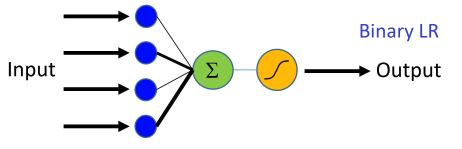
\includegraphics[width = \textwidth]{images/logistic_reg.png}
\caption{Wiginton's Logistic Regression Model}
\parencite{LogRegFig}
\label{fig:LR}
\end{figure}

\vspace{15pt}

Wiginton deemed that a logistic regression model gave superior classification results when compared to a LDA model. His model was able to achieve a classification accuracy of over 58\%. However, \textcite{LogRegHand} compared using logistic regression approach to simple linear regression and found that both approaches had very similar classification accuracies. 

\subsection{Classification Tress}

Classification and Regression Trees (CART) are another statistical technique that have been commonly used for credit scoring. Like LDA and logistic regression, they have been used to classify potential borrowers into either a "likely to repay a financial obligation" or "unlikely to repay a financial obligation" class. They are non-parametric models used to predict a dependent variable as a function of continuous independent variables. Decision trees are dichotomous models that are developed by splitting the records at each node based on a function of a single input. They consider all possible splits and identify the best sub-tree based on its overall error rate \parencite{DecTreesZekic}. \\

The CART algorithm was developed by \textcite{DecTreesBrieman}. They found that CART models are invariant under transformations in the predictor space and that Multi-factor response is easily dealt with. Furthermore, they found that modelling results could be easily to explained to non-statisticians due to their CART's inherent visual properties. Figure \ref{fig:CART} displays the algorithm developed by \textcite{DecTreesBrieman}. 

\vspace{15pt}

\begin{figure}[!htb]
\centering
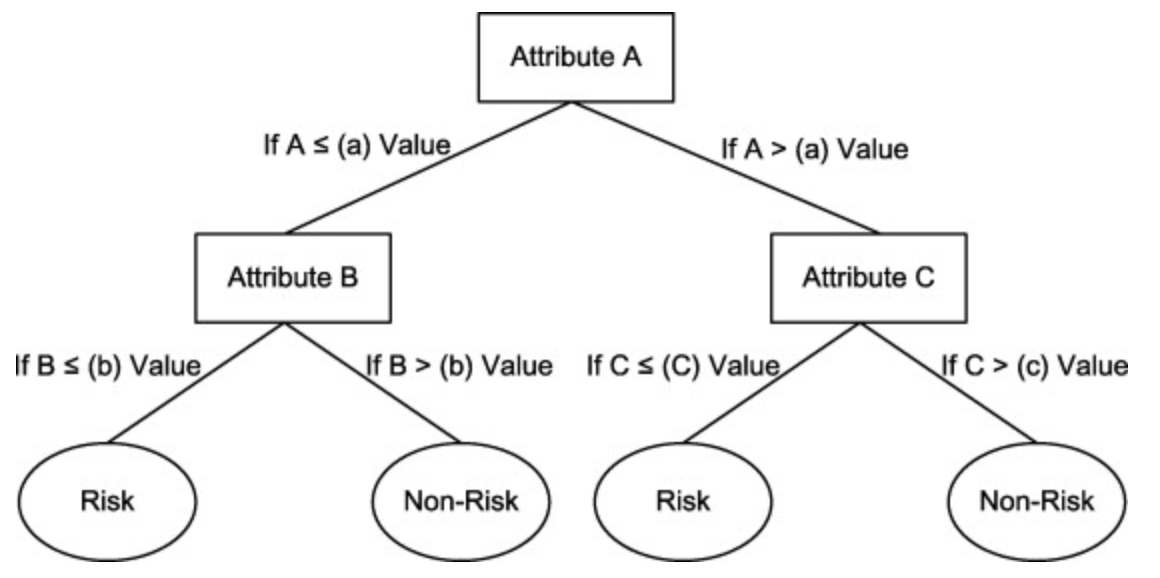
\includegraphics[width = \textwidth]{images/CART.png}
\caption{CART Model}
\parencite{DecTreesBrieman}
\label{fig:CART}
\end{figure}

\vspace{15pt}

In figure \ref{fig:CART} the subset branches created by each split are ref referred to as nodes. The subsets which are not split are named terminal nodes. Terminal nodes get assigned to one of the predefined classes. In figure \ref{fig:CART} there are 3 classes. A predicted classes for an input vector is found by passing through each binary node in the tree until a terminal node is reached. \\

\textcite{DecTreesZekic} compared the performance of a CART, a neural network (NN) and logistic regression model in scoring a sample small business loans provided by a Croatian bank. They used pruning to avoid over-fitting. A technique that involves growing a tree and then removing branches and terminal nodes that do not contain a predefined number of data points. They used Gini index as the evaluation function used for splitting. \newpage


Gini index is calculated as shown in equation \ref{eq:GINI}. 

\vspace{15pt}

\begin{equation} \label{eq:GINI}
\sum_{j!=k}p_{ij}p_{ik} = 1 - \sum_{k}p_{ik}^{2}
\end{equation}
\vspace{15pt}

Where p represents the independent variables. \\


The results of \textcite{DecTreesZekic} research can be seen in table \ref{table:CART}. \\


\begin{table}[H]
\begin{center}
\begin{tabular}{|c|c|c|c|} 
\hline
\multicolumn{1}{|c}{Model}  &\multicolumn{1}{|c|}{Total Accuracy (\%)}  &\multicolumn{1}{|c|}{Bad Accuracy (\%)} & \multicolumn{1}{c|}{Good Accuracy (\%)}\\
\hline
Probabilistic NN & 83.30 &  80.00 & 85.19 \\
\hline
Logistic regression & 57.14 &  66.67 & 51.85 \\
\hline
CART & 66.67 &  66.67 & 66.67 \\
\hline
\end{tabular}
\end{center}
\caption{Results of Research Conducted by \textcite{DecTreesZekic} }
\label{table:CART}
\end{table}

\vspace{15pt}

The models displayed in Table \ref{table:CART} were trained on the same training data and the same 20 variables. It can be seen from Table \ref{table:CART} that the CART model produced by \textcite{DecTreesZekic} outperformed their logistic regression model in terms of total accuracy and in terms of predicting loans that were repaid (Good Accuracy). However, the CART model was outperformed in predicting both loan that were not repaid (Bad Accuracy), loans there were not repaid and over all accuracy by their probabilistic NN model.  

%---------------------------------------------------------------------------------------
%	SECTION 3
%---------------------------------------------------------------------------------------
\section{Machine Learning Models}

After the rapid expansion of consumer credit numerous statistical methods were successfully used for credit risk assessment. However, these models often had difficulty in modelling complex financial scenarios due to their use of fixed functions and statistical assumptions \parencite{AICredDefSwap}. Studies have shown that machine learning techniques such as Support Vector Machines (SVM's), Random Forests , and Neural Networks are superior to that of statistical techniques in terms of predicting whether consumers are likely to repay a loan when the training sample is large \parencite{SVMCrook}. 


\subsection{Support Vector Machines}

SVM models define a hyper-plane that best separates two data classes so that the margin width between the hyper-plane and
the data points is maximised. The hyper-plane can be linear or non-linear. The wider the  margin width, the less complex the model is and the more likely it is to generalise well. \\


The hyper-plane can often be difficult to define if the classes are not well separated. Figure \ref{fig:SVM} displays such a case. \newpage

\vspace{15pt}

\begin{figure}[!htb]
\centering
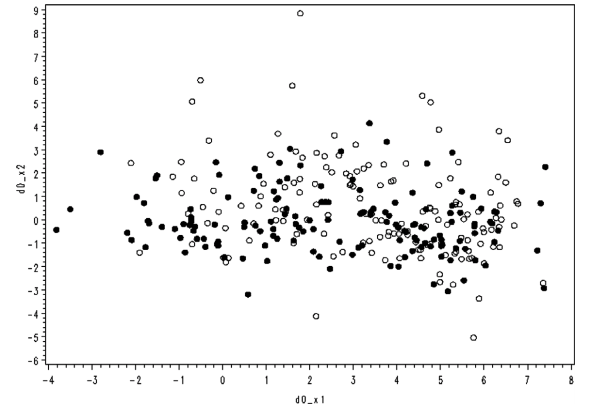
\includegraphics[width = 0.9\textwidth]{images/SVM.png}
\caption{Poorly Separated Credit Data}
\parencite{SVMCrook}
\label{fig:SVM}
\end{figure}

\vspace{15pt}


\textcite{SVMCrook} developed a SVM model that predicted whether credit card users would default on their repayments. A consumer was deemed to have defaulted if they fell more than 3 months behind on their repayments within the first 12 months of their account opening. They used a training sample of 25,000 consumers. The model developed used a a non-linear kernel and its parameters were tuned using a grid search in order to maximise the model's area under the Receiver operating characteristic curve (AUC), which is a single summary statistic used to measure a binary classification model's specificity (true negative rate) and sensitivity (true positive rate). \\

On top using the SVM model to classify loans, \textcite{SVMCrook} used the magnitude of the weight of each feature as a feature selection criterion. They only included features with a weight of more than 0.1 in their final model. They compared their SVM model to a logistic regression and k-nearest neighbours (KNN) model. They compared each model's AUC, sensitivity and specificity. Figure \ref{fig:SVMLR} compares the performance of SVM model to the performance of the logistic regression model, while figure \ref{fig:SVMKNN} compares the performance of SVM model to the performance of the KNN model. In both figures the solid line is the SVM model's performance and the broken line is the other model. \\

We can see from figures \ref{fig:SVMLR} and \ref{fig:SVMKNN} that the SVM model outperformed the other model. Furthermore, the SVM model had a better training and test AUC, specificity , and sensitivity than the other two models. 

\vspace{15pt}

\begin{figure}[!htb]
\centering
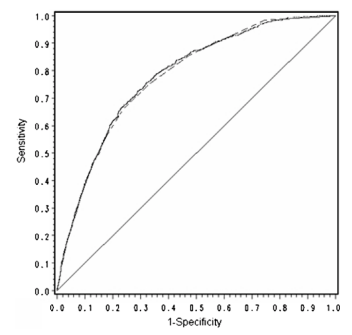
\includegraphics[width=0.7\textwidth]{images/SVMLR.png}
\caption{SVM Model vs Logistic Regression Model}
\label{fig:SVMLR}
\end{figure}

\begin{figure}[!htb]
\centering
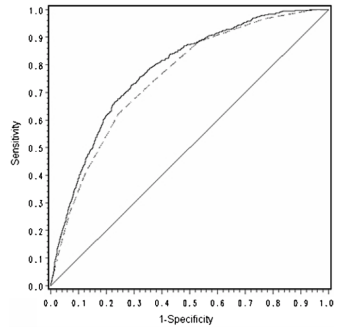
\includegraphics[width=0.7\textwidth]{images/SVMKNN.png}
\caption{SVM Model vs KNN Model}
\label{fig:SVMKNN}
\end{figure}

\vspace{15pt}

\subsection{Neural Networks}

The research conducted by \textcite{DecTreesZekic} displayed that neural networks improved on classification accuracy of more traditional statistical techniques such as decision trees and logistic regression when classifying whether or not consumers would repay a financial obligation. The research conducted by \textcite{NNWest} compared the performance, of five different neural network models, when they are applied to credit scoring.  The models developed varied in architecture, loss functions, and learning rates.  \\

West developed models with the following features: a multi-layer perceptron (MLP) model, a model that used the mixture-of-experts (MOE) approach, a model that used a radial basis function (RBF), learning vector quantization (LQV) model, and fuzzy adaptive resonance (FAR) model. The architectures of each model were made similar. The input and of and output layers of each model were identical. However, the hidden layer of each model varied. West determined the optimal number of nodes in the hidden layer of the MLP and MOE models using a cascade learning approach. The hidden layer layer of the LQV model was determined by setting the number of neurons in the layer equal to 10\% of the size of the training data. The hidden layers of the RBF and RAF models were determined experimentally.  \\

West used a sample of 1000 loans, provided by a German credit provider, to train and test the models he developed. The sample consisted of 700 loans that were repaid and 300 that were not. He used the same features to train each model and used 10-fold cross validation to test the accuracy of each model. 10-fold cross validation involves partitioning the training sample of a model into 10 partitions. One partition serves as an independent holdout test set for the credit model being trained while the remaining nine partitions are used to train the model. This technique minimises the effects of data dependencies and improves the reliability of the estimates. \\

Table \ref{table:NN} displays the results of West's research. Like Table \ref{table:CART}, Table \ref{table:NN} displays each model's accuracy in terms of predicting loans that were repaid, loans that were not repaid ,and overall prediction accuracy. The accuracies show are the average of the best three results from the 10-fold cross validation conducted for each model. 

\vspace{15pt}

\begin{table}[H]
\begin{center}
\begin{tabular}{|c|c|c|c|} 
\hline
\multicolumn{1}{|c}{Model}  &\multicolumn{1}{|c|}{Total Accuracy (\%)}  &\multicolumn{1}{|c|}{Bad Accuracy (\%)} & \multicolumn{1}{c|}{Good Accuracy (\%)}\\
\hline
MLP & 87.09 &  46.92 & 75.04 \\
\hline
MOE & 86.99 &  55.43 & 77.57 \\
\hline
RBF & 85.76 &  51.79 & 75.63 \\
\hline
LQV & 79.15 &  55.20 & 72.20 \\
\hline
FAR & 70.92 &  58.14 & 62.29 \\
\hline
\end{tabular}
\end{center}
\caption{Results of Research Conducted by \textcite{NNWest}}
\label{table:NN}
\end{table}

\vspace{15pt}

Table \ref{table:NN} displays that the MOE model is the best overall performing model. \textcite{NNWest} used a chi-square test to assess whether or not there were significant differences between the models he developed in terms of predicting loan default. The chi-square test indicated that MOE, RBF, and MLP are superior models for predicting loan repayment when compared to RAF and LQV models. \\

Table \ref{table:NN} does not show that West developed logistic regression and CART models as reference models. These models outperformed all neural network models, but were deemed significantly similar to the MOE, RBF, and MLP models. The reason for the strong performance of the statistical approaches was deemed to be due to the size of training set used to develop the models.  \\

\textcite{NNShen} used the same dataset as \textcite{NNWest} to train and test a back propagated neural network. Their model used a particle swarm optimisation (PSO) algorithm to search for the optimal weights and deviations in the BP neural network. \\

Further more, they used synthetic minority over-sampling technique (SMOTE) to balance the training dataset before the training the model. This was done as the majority of  credit history datasets are imbalanced towards the class containing customers that repaid their financial obligations. SMOTE involves generating synthetic examples of data points that belong to the minority class in a training dataset. \textcite{NNShen} generated synthetic examples by identifying the k nearest neighbours of a randomly selected minority data point. A variable difference vector between the minority instance under consideration and its corresponding nearest neighbours was then calculated and multiplied using a by a random value between 0 and 1. The feature vector was then added to the original minority data point. This process was completed until the ratio of credit defaulters and credit re-payers matched. Figure \ref{fig:smote} visually displays the steps carried out in the class balancing process. 

\vspace{15pt}

\begin{figure}[!htb]
\centering
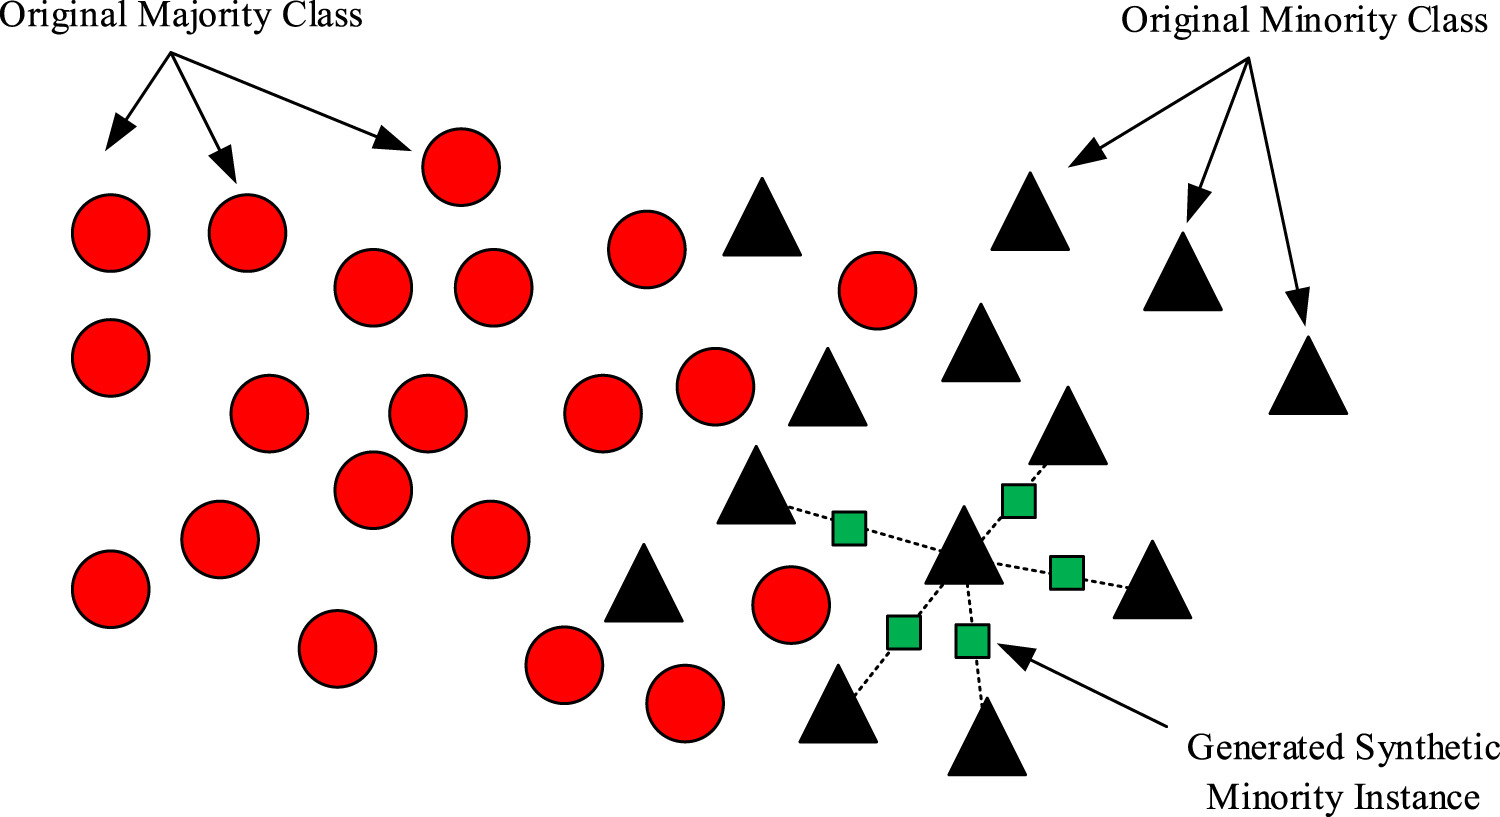
\includegraphics[width=0.7\textwidth]{images/smote.jpg}
\caption{Synthetic Minority Over-Sampling Technique}
\parencite{NNShen}
\label{fig:smote}
\end{figure}

\vspace{15pt}

\textcite{NNShen} compared their back propagation NN, with PSO weight determination, model against 7 other techniques. These techniques included LDA, logistic regression (Log R in Figure \ref{fig:shen}), SVM, a back propagation NN that did not use the PSO weight determination method (BP in Figure \ref{fig:shen}), KNN, classification trees (CT in Figure \ref{fig:shen}), and a Naive Bayes classifier (NB in Figure \ref{fig:shen}). Each model was trained on the same balanced dataset. Like \textcite{NNWest}, \textcite{NNShen} used 10-fold cross validation to test each developed model. Figure \ref{fig:shen} displays that their model out performed the other models in AUC, total accuracy, F1-score, and repaid accuracy (Type I Accuracy in the figure). The model did however not outperform all models in detecting defaulted credits (Type II Accuracy in the figure). 

\vspace{15pt}

\begin{figure}[!htb]
\centering
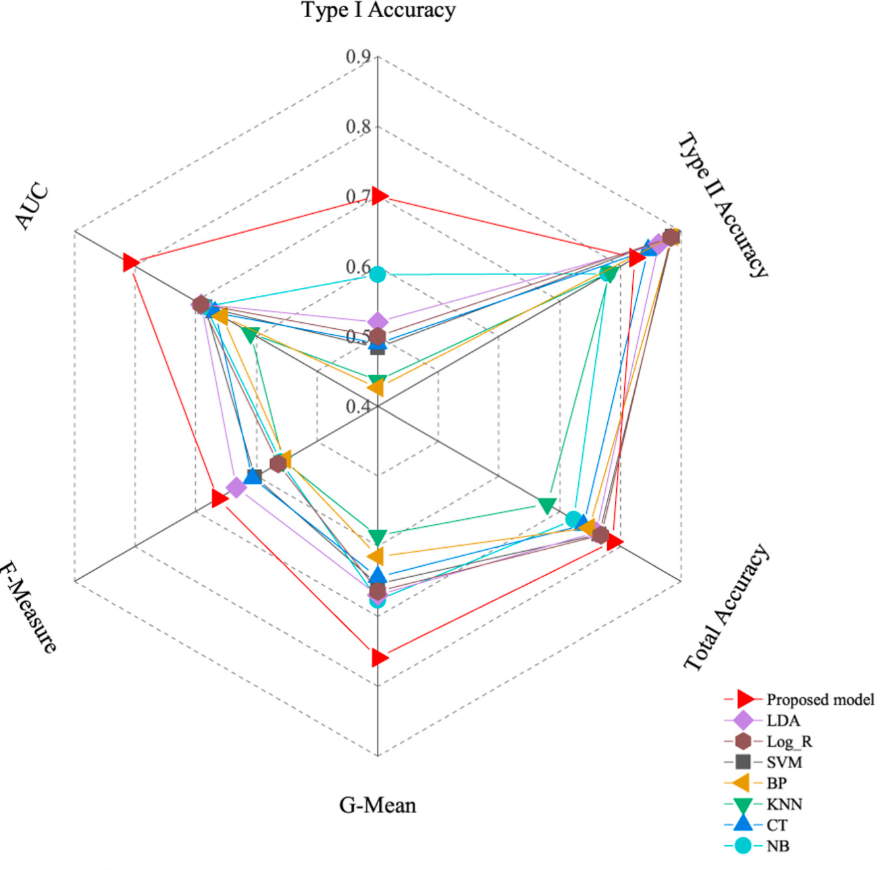
\includegraphics[width=0.7\textwidth]{images/shen.png}
\caption{The Results of the Research Conducted by \textcite{NNShen}}
\label{fig:shen}
\end{figure}

\vspace{15pt}

%---------------------------------------------------------------------------------------
%	SECTION 4
%---------------------------------------------------------------------------------------

\section{Ensemble Models}

There are two main methods used for ensemble modelling. The first is a parallel structure, which involves developing more than one model from training data and combining their outputs based on an ensemble strategy to produce a final prediction. The second method is a consequential structure, which involves feeding the output of one model into the next until a final outcome is produced. Figure \ref{fig:ensemble} visually displays the two main methods. 

\vspace{15pt}

\begin{figure}[!htb]
\centering
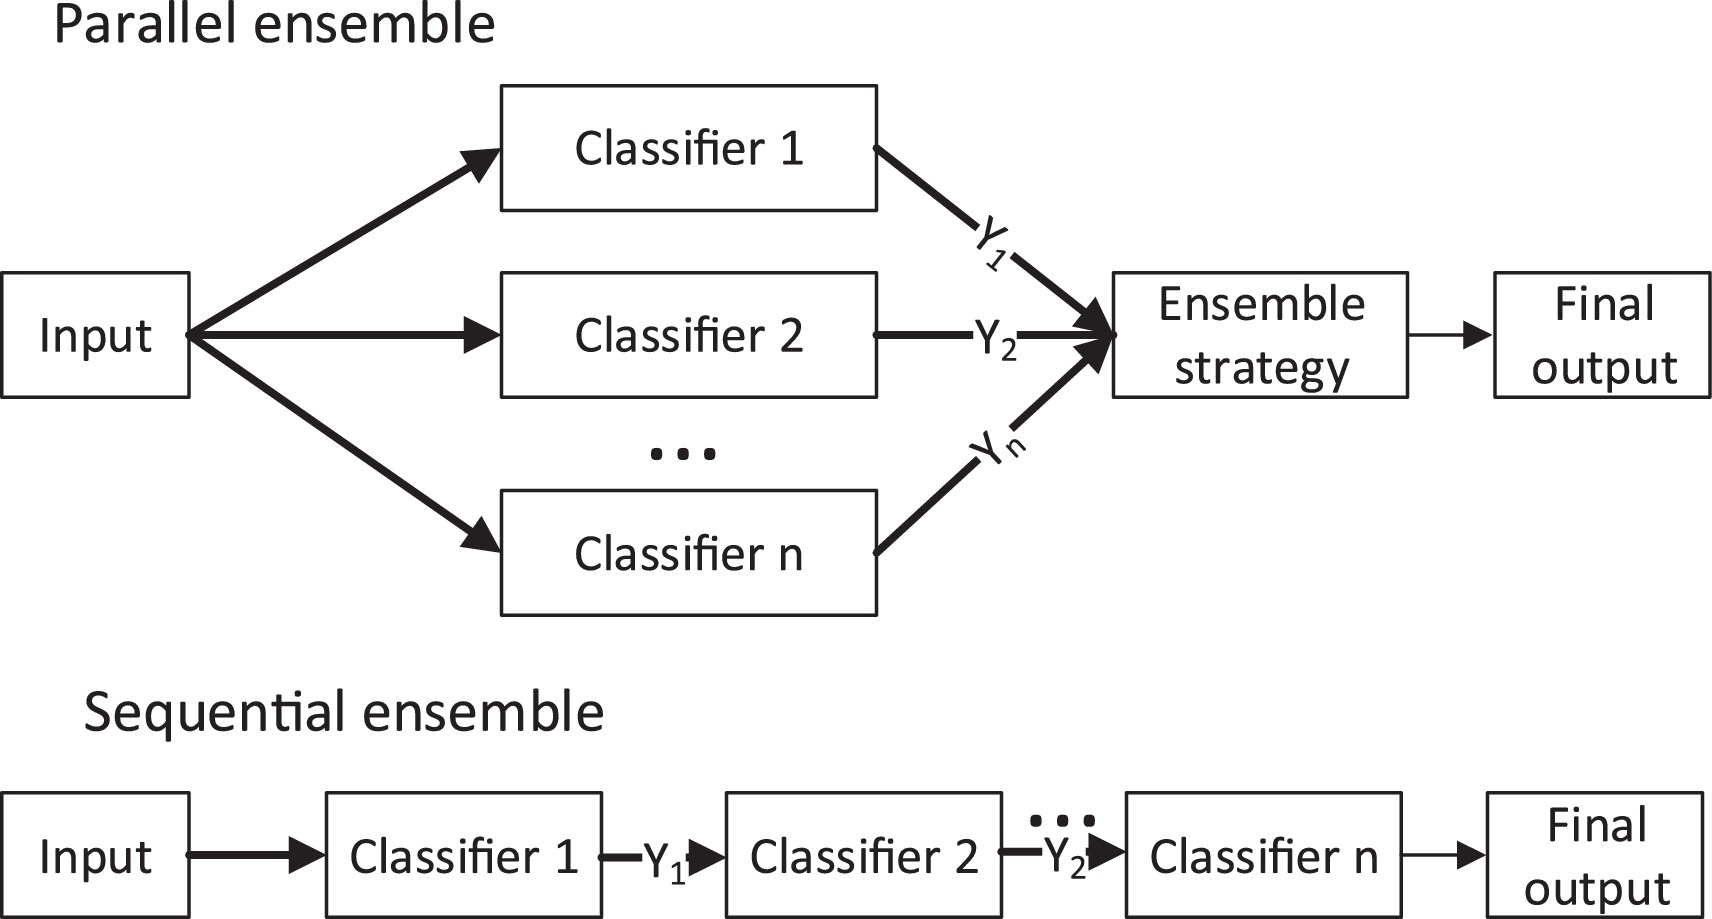
\includegraphics[width=0.6\textwidth]{images/ensemble.jpg}
\caption{Parallel and Consequential Ensemble Models}
\parencite{Ensemble}
\label{fig:ensemble}
\end{figure}

\vspace{15pt}

\subsection{Bagging}

Bootstrap aggregating is one of the earliest parallel ensemble machine learning methods. It was first developed by \textcite{BagBri}. The method involves developing numerous base models of the same underlying structure. Each model is trained on a separate sub-dataset that is randomly drawn—with replacement—from the entire dataset. The models are combined using majority vote. \\

\textcite{BagWang} developed a bagging credit scoring model that used decision trees as the underlying base models. In order to further improve the performance of their model and to avoid redundant features impacting the model, when each new decision tree was trained on a sub-dataset not all features available features were used. Features were randomly sampled. This feature sampling technique is referred to as random subspace sampling. \\

\textcite{BagWang} used the same German credit provider dataset used by \textcite{NNWest} and \textcite{NNShen} to train their model. \textcite{BagWang} further developed a decision tree model, a random forest model, and a bagging model that did not make use of random subspace sampling for comparative purposes. The results from their research can be seen in Table \ref{table:bagging}. 


\vspace{15pt}

\begin{table}[H]
\begin{center}
\begin{tabular}{|c|c|c|c|} 
\hline
\multicolumn{1}{|c}{Model}  &\multicolumn{1}{|c|}{Total Accuracy (\%)}  &\multicolumn{1}{|c|}{Bad Accuracy (\%)} & \multicolumn{1}{c|}{Good Accuracy (\%)}\\
\hline
DT  & 72.10 &  46.80 & 72.94 \\
\hline
Random Forest & 77.05 & 43.72 & 90.48 \\
\hline
Bagging & 78.36 & 41.44 & 94.02 \\
\hline
Bagging with RS & 78.52 &  44.66 & 92.81 \\
\hline
\end{tabular}
\end{center}
\caption{Results of Research Conducted by \textcite{BagWang}}
\label{table:bagging}
\end{table}

\vspace{15pt}

Table \ref{table:bagging} displays that the bagging model that used random subspace sampling (RS) outperformed the other models in overall classification accuracy. It is interesting to note that although the decision tree model had the lowest overall accuracy, it performed best in terms of classifying loans that were not repaid (true negatives). Table \ref{table:bagging} further displays that all models developed by \textcite{BagWang} had low specificity (classifying loans that were not repaid as bad loans) rates. 


\subsection{Boosting}

Boosting is a sequential ensemble machine learning technique that involves altering the weights of samples in training datasets based on the errors of previously created classifiers. Misclassified samples in the training set are assigned with higher weights. A weighted voting scheme is then applied to produce a final model \parencite{BoostingFreund}. \\

\textcite{Ensemble} used extreme gradient boosting (XGBoost) to develop a credit repayment classification model. New base models in the XGBoost algorithm predict the residuals of previous base models in the sequence and add the outputs of each model are then added together to produce a final prediction. The algorithm uses gradient descent to minimise a defined loss function \parencite{BoostingCowan}. \\

The base models used in \textcite{Ensemble} were decision trees. The hyper-parameters of their XGBoost model were adaptively tuned using Bayesian optimisation, which involved mapping each hyper-parameter to the loss function and iteratively finding the local hyper-parameter function which minimised the loss function of the XGBoost model. \\

They further developed baseline models and used other hyper-parameter tuning methods to assess the performance of the model they developed. The XGBoost model developed outperformed bagging, decision tree, logistic regression, neural network, random forest and support vector machine models in overall prediction accuracy, area under the curve, and Brier score. Furthermore, the XGBoost model developed using Bayesian hyper-parameter optimisation outperformed 4 XGBoost models in overall prediction accuracy, area under the curve, and Brier score that used a grid search, a manual search and a random search algorithm to tune their hyper-parameters respectively. All models developed by \textcite{Ensemble} were trained on five separate credit datasets. The metrics presented were an aggregation of each model's performance across all datasets. \\


%---------------------------------------------------------------------------------------
%	SECTION 5
%---------------------------------------------------------------------------------------

\section{Alternative Data in Credit Scoring}


In the decade between 1998 and 2008, the number of micro-finance institutions (MFIs) grew by 474\% and their number of customers increased by over 1000\%. MFIs generally provide a low amount, short term loans to lower income individuals. In less developed countries many first time customers for MFIs belong to the world's unbanked population. Furthermore, the credit bureaus in less developed countries do not necessarily store and release accurate and reliable data on the banked population. Traditional credit scoring models can therefore not always be applied to in these regions \parencite{MFICinca}.  \\


\textcite{MFIMLP} developed a multi-perceptron neural network that was trained on over 5,400 loans provided by Peruvian MFIs. The model used features that related to the personal characteristics of the loanees, the economic and financial ratios of the MFI the loan was provided by, the characteristics of the financial obligation (interest rate of loan, loan amount etc.), and variables related to the macroeconomic climate of Peru during the time time period of the loan. \\


\textcite{MFIMLP} developed a LDA model, logistic regression model, and multiple MLP models with varying architectures for comparative purposes. The architecture which lead to the most accurate MLP model was a 3 layer perceptron with 20 input nodes, 3 hidden nodes and a single output node. Each model was trained and its parameters tuned using 10-fold cross-validation. Table \ref{table:MFIMLP} displays the results of the LDA model, logistic regression and most accurate MLP models. 

\vspace{15pt}

\begin{table}[H]
\begin{center}
\begin{tabular}{|c|c|c|c|c|} 
\hline
\multicolumn{1}{|c}{Model}  &\multicolumn{1}{|c|}{AUC}  &\multicolumn{1}{|c|}{Bad Accuracy (\%)} & \multicolumn{1}{c|}{Good Accuracy (\%)} & \multicolumn{1}{c|}{Misclassification Costs}\\
\hline
LDA  & 0.9303 &  81.73 & 93.48 & 0.5143 \\
\hline
LR & 0.9322 & 79.04 & 94.06  & 0.5715 \\
\hline
MLP & 0.9543 & 84.70 & 92.24 & 0.4337 \\
\hline
\end{tabular}
\end{center}
\caption{Results of Research Conducted by \textcite{MFIMLP}}
\label{table:MFIMLP}
\end{table}

\vspace{15pt}

It can been seen in Table \ref{table:MFIMLP} that the MLP model has the highest AUC, the lowest misclassification cost and has the highest accuracy in terms of identifying loans that were not repaid as bad loans. \\

\textcite{BigDataMicroFiance} investigated the use of alternative
data sources to enhance the statistical and economic  performance of credit scoring models. They measured the impact of augmenting typical scoring features with features generated from cell phone data. The credit data was provided by a banking institution and the cell phone data was provided by a telecommunications provider. The data provided by the bank contained sociodemographic, account data and credit card repayment data for over 2 million customers. The data provided by the telecommunications company consisted of call data for over 90 million unique cell phone users. \\

Both data sources were used to generate a connected network between customers of both companies. Figure \ref{fig:network} displays an overall view of the network. Creditors were deemed to be a defaulter if they had missed 3 or more credit card repayments. 

\vspace{15pt}

\begin{figure}[!htb]
\centering
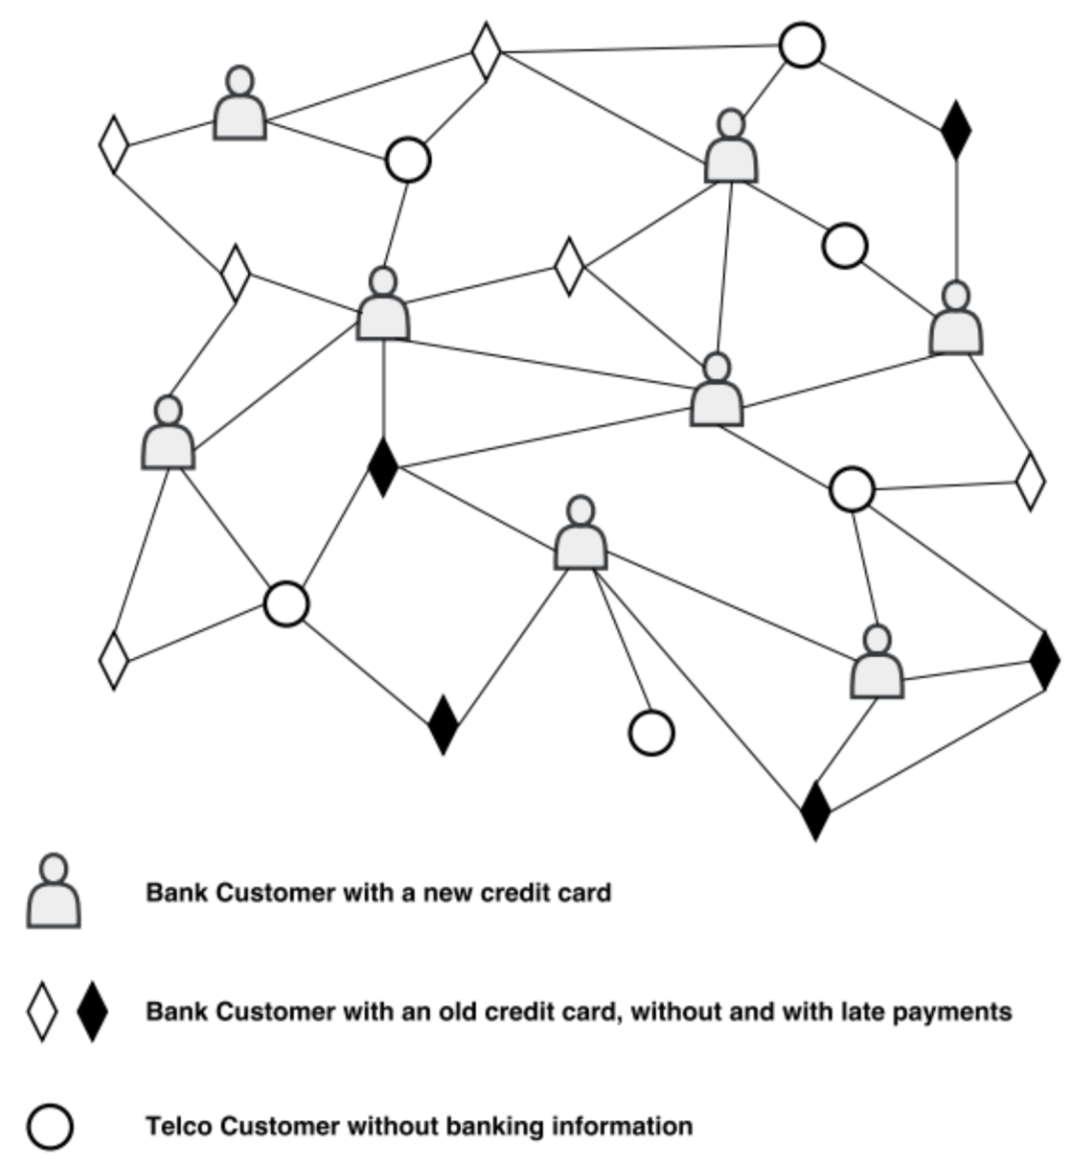
\includegraphics[width=0.6\textwidth]{images/network.png}
\caption{Network of Bank and Telecommunications Customers}
\parencite{BigDataMicroFiance}
\label{fig:network}
\end{figure}

\vspace{15pt}

 There were a total of 3 networks developed. One for each month that credit cards were disbursed to bank's customers. Bank customers and telecommunications customers that had shared a phone call within the three whole month period prior to the card acquisition month were connected. For each network \textcite{BigDataMicroFiance} used network analytics techniques to  propagate the influence of related defaulters throughout the network to produce influence scores. \\
 
 The call data features extracted from the network were as follows; the number and duration of incoming, outgoing and undirected phone calls taking place during the day and night and on different days of the week were computed. Furthermore, exposure scores to defaulted clients were calculated for each customer of each network using Personalised PageRank (PR) and Spreading Activation (SPA). \\
 
 
\textcite{BigDataMicroFiance} features listed above were combined with demographic and account data provided by the bank to build a credit scoring model for sample of bank's customers. This sample included only 22,000 of the banks 2 million customers. A logistic regression model, a decision tree model and a random forest model were developed for different feature samples. A sample was used that only contained sociodemographic (SD) features, another that only used credit based (CB) features, one that used both SD and CB features, one that used CB features and alternative features generated from the call data and network analysis, and finally one that used SD, CB, and alternative features generated from the call data and network analysis. The AUC of the different feature samples and models can be seen in Table \ref{table:alt}. 

\vspace{15pt}

\begin{table}[H]
\begin{center}
\begin{tabular}{|c|c|c|c|} 
\hline
\multicolumn{1}{|c}{Features}  &\multicolumn{1}{|c|}{Logistic regression}  &\multicolumn{1}{|c|}{Decision Trees} & \multicolumn{1}{c|}{Random Forest}\\
\hline
SD only  & 0.5869 &  0.7004 & 0.8993  \\
\hline
CB only & 0.5351 & 0.7043 & 0.8700  \\
\hline
SD and CB & 0.6115 & 0.7127 & 0.9227  \\
\hline
CB and Alternative & 0.5182 & 0.7307 & 0.0.9154  \\
\hline
SD,CB and Alternative & 0.6121 & 0.7263 & 0.9224  \\
\hline
\end{tabular}
\end{center}
\caption{Results of Research Conducted by \textcite{BigDataMicroFiance}}
\label{table:alt}
\end{table}

\vspace{15pt}
 
 
It can been seen in Table \ref{table:alt} that the performance of each
model type varies substantially. Furthermore, the logistic
regression models did not perform better when the
network-related features were used. This was believed to be due to linear regression models not being able to capture the non-linear behaviour of the network-related features. The best performing models were the random forest models. \\

The AUC test devised by \textcite{AUC} was used by \textcite{BigDataMicroFiance} to compare the performance of the random forest models. It was discovered that at a 95\% confidence level, the model produced both SD and CB features, the model produced using CB features and alternative features generated from the call data and network analysis, and the model produce using SD, CB, and alternative features showed a a significant statistical improvement in model performance compared to the models that used only SD and CB features.\\

However, there was no statistical difference between the model that used  SD and CB features, the model produced using CB features and alternative features generated from the call data and network analysis, and the model produce using SD, CB, and alternative features. 

\chapter{Data Extraction and Preprocessing} 
\label{Chapter3}

This chapter details the data sources used to train the various credit scoring models developed throughout this project, the various data extraction techniques used to extract the alternative data features within the training sets, and the pre-processing and feature engineering techniques deployed before the modelling phase.   
%---------------------------------------------------------------------------------------
%	SECTION 1
%---------------------------------------------------------------------------------------

\section{Data Used}

\subsection{Sources}

There were two main data sources used to train the models developed throughout this project. The first data source is a Nigerian micro-finance institution that has disbursed loans to more than 250,000 consumers. The institution is an application-based lender and currently only disburses to android users. The institution, with its customers' consent, gains access to the data on customers' devices. This data includes SMS data, contact data and location data. On top of the alternative data collected, sociodemographic data is collected via customer input on the institution's application. \\

The second data source used was the Nigerian credit bureaus CRC, CRS and XDS. It is mandatory for credit providing institutions in Nigeria to submit their customers' credit performance data to these credit bureaus. \\

A final dataset was created for first time loan customers of the micro-finance institution that had existing credit bureau data prior to their first application. The customers required existing credit data as it was needed in order to compare the performance of first time credit credit scoring models that use only alternative data or alternative data in conjunction with sociodemographic data, against first time credit scoring models that make use of existing credit data. The final dataset consisted of 49,550 customers/loans. 

\subsection{Data Categories}

Three major data categories were drawn from the data sources. These categories were sociodemographic data, credit bureau data and alternative data. The main aim of this thesis is to assess how alternative data can augment traditional credit scoring data. To complete this aim various combinations of these data categories were used to develop various credit scoring models. The statistical performance of the models were assessed in order to test whether using the various data categories resulted in a significant difference in model performance. 

%---------------------------------------------------------------------------------------
%	SECTION 2
%---------------------------------------------------------------------------------------

\section{Data Extraction and Feature Engineering}

\subsection{Sociodemographic and Credit Bureau Data}

The more traditional credit scoring features, developed from sociodemographic and credit bureau data attached to each first-time borrower, were created and extracted using SQL (Structured Query Language). The data was extracted from the company's relational database. \\

The query was written in a manner that ensured that no data leakage would occur when the credit scoring models were being trained. This means that only data that would be known at the point in time when a particular client applied for their loan could be sued to develop features. The only case were data was used that would not be known at the point in time of application was repayment data, as this was used to develop the default (whether the client repaid their loan or not) target variable. \\

The overall query used to extract the sociodemographic and credit bureau for each loan was a collection of sub-queries joined on a unique key attached to each loan. The query used to extract the credit bureau required an aggregation in order to generate features that represented the total number of loans each client had prior to their application with the micro-finance institution used in this study. The credit bureau features used in the modelling process and their definitions can be found in the appendix of this paper. The sociodemographic data was extracted using a simpler sub-query,  like the credit bureau features their definitions can be found in the appendix of this paper.  \\


\subsection{Alternative Data}

The three main sources of alternative data used to develop features were the application, SMS, and device data stored on each customers' cellphone. The data was extracted from the micro-finance institution's using PyMongo, a Python package that allows a user to query data from a Mongo database from within a Python script. The application and SMS data was extracted from different Mongo databases, however expressions (regex) were used to filter both data types and to develop features. Regex functions are sets of sequences of characters that define a particularly search pattern. The functions are then used to identify cases of the defined pattern in strings \parencite{Regex}. \\

The device data was extracted from a separate database as the application and SMS data and an entirely different technique was used to generate features from the data. The technique used in this case was web scraping, which is a method of extracting data from websites \parencite{WebScraping}. 

\subsubsection{Application Based Features}

The application based features engineered for this project were counts of particular applications present on a clients device at the point in time of their application. The features included a count of the finical, competing micro-finance, news, gambling and virtual private network (VPN) applications. The counts were generated by first compiling a list of all unique applications on a client's. Then the name of each application was passed through a series of regular expression key word searches. Each expression was designed to detect a specific application type. If  a particular application type search resulted in a match, the count associated with that search was updated. \\

The process developed to pass an application through the application extracting regular expressions and how the count features were generated throughout this process is represented in Figure \ref{fig:app_features}. The process was coming up ompleted for every unique application recorded on the client's device. 


\vspace{15pt}

\begin{Figure}[!htb]
\centering
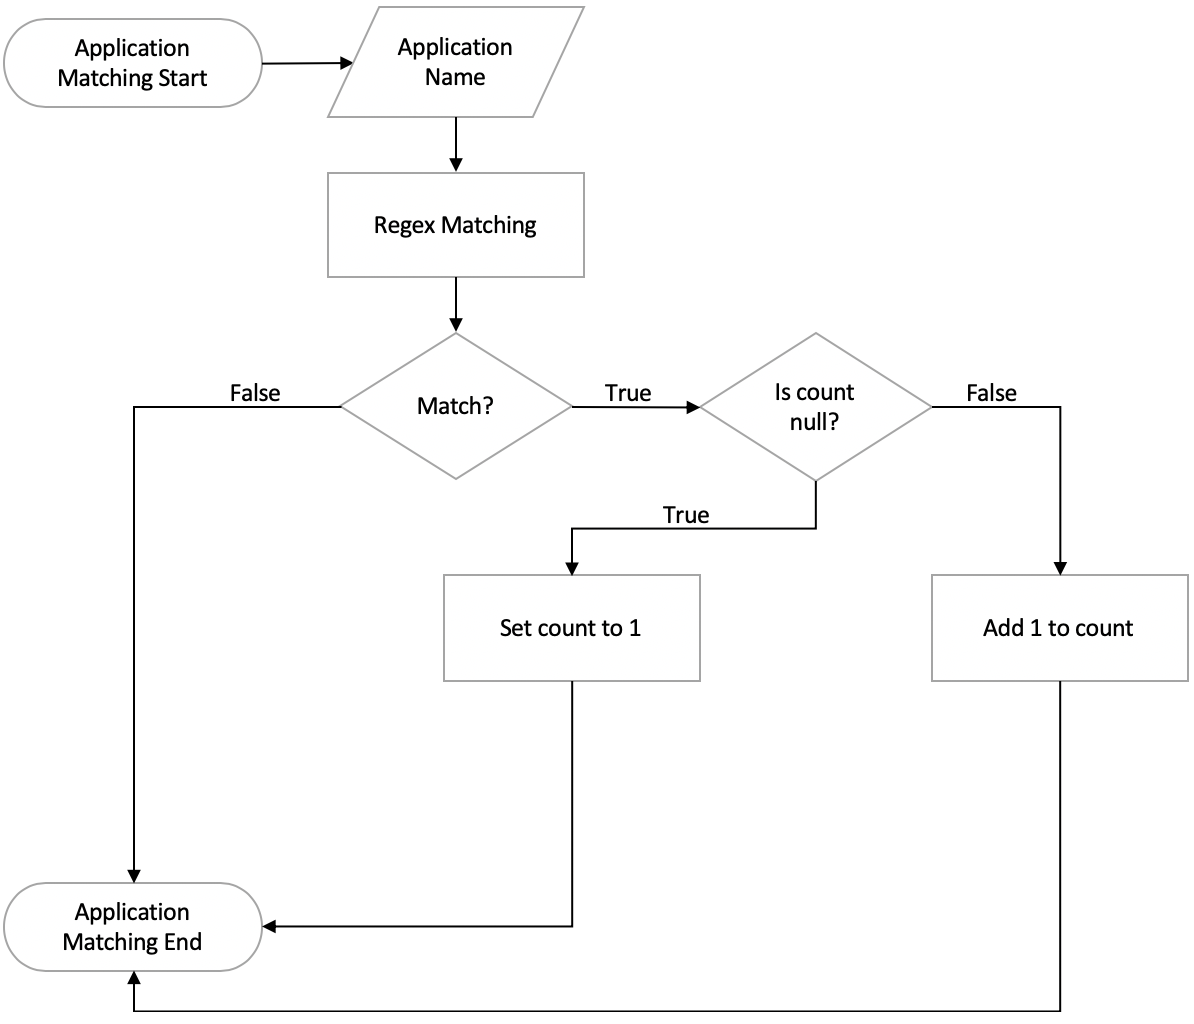
\includegraphics[width=0.6\textwidth]{images/app_feats.png}
\caption{Application Based Feature Generation}
\label{fig:app_features}
\end{Figure}

\vspace{15pt}


\subsubsection{SMS Based Features}

The SMS data consisted of messages received by the clients in the 90 days prior to their application, by nature this data is more sensitive than the other data used throughout this research. Similarly to the process developed to generate the application based features, each message received by a client was complied into a list. The list was the looped over in order to generate features for each application/client. \\ 

In order to avoid exposing personal messages the each message was passed through two filtering regular expressions. The first expression returned only messages received from Nigerian banks, while the second ensured that only messages returned by competitor micro-finance institutions were returned. The regular expressions had a dual purpose. They prevented exposure to sensitive content and they acted as the first step in the SMS based feature generation process. \\

If a messaged passed through the regular expression for banking messages it was exposed to the banking feature creation process. Typically, messages from Nigerian banks have a similar structure. They display a transaction amount, the date of the transaction, the type of transaction (credit or debit to the account), and finally the balance in the account after the transaction. Regular expressions were used to identify the type of transaction, extract the transaction amount and extract the account balance. The transaction amounts were then appended to lists.  \\

If a message did not pass through the banking regular expression it was then passed to the competitor expression. If the message passed through this expression it was then further screened by another set of regex functions. These functions searched for key words in order to identify if a client had another loan with a competitor and if that loan had been repaid successfully or not. The actual loan amount was extracted using regex as was the loan repayment (instalment amount). These amounts were appended to lists. \\

After the passing every message associated to a particular client through the regex functions the lists created throughout the process were used to generate the SMS based features for that particular client. \\

The banking related features generated were:

\begin{itemize}
    \item The number of unique banks that sent the client a message
    \item The minimum and maximum debit transaction, credit transaction and account balance values extracted
    \item The total number of debit and credit transactions recorded
    \item The number of times the term 'insufficient funds' was recorded in the client's messages
\end{itemize}

\vspace{15pt}

The process of passing an SMS through the bank related regular expressions and how the banking features were generated throughout that process is represented in Figure \ref{fig:bank_features}. The process was completed for every message received by a client within the 90 day period prior to their application. 

\vspace{15pt}

\begin{Figure}[!htb]
\centering
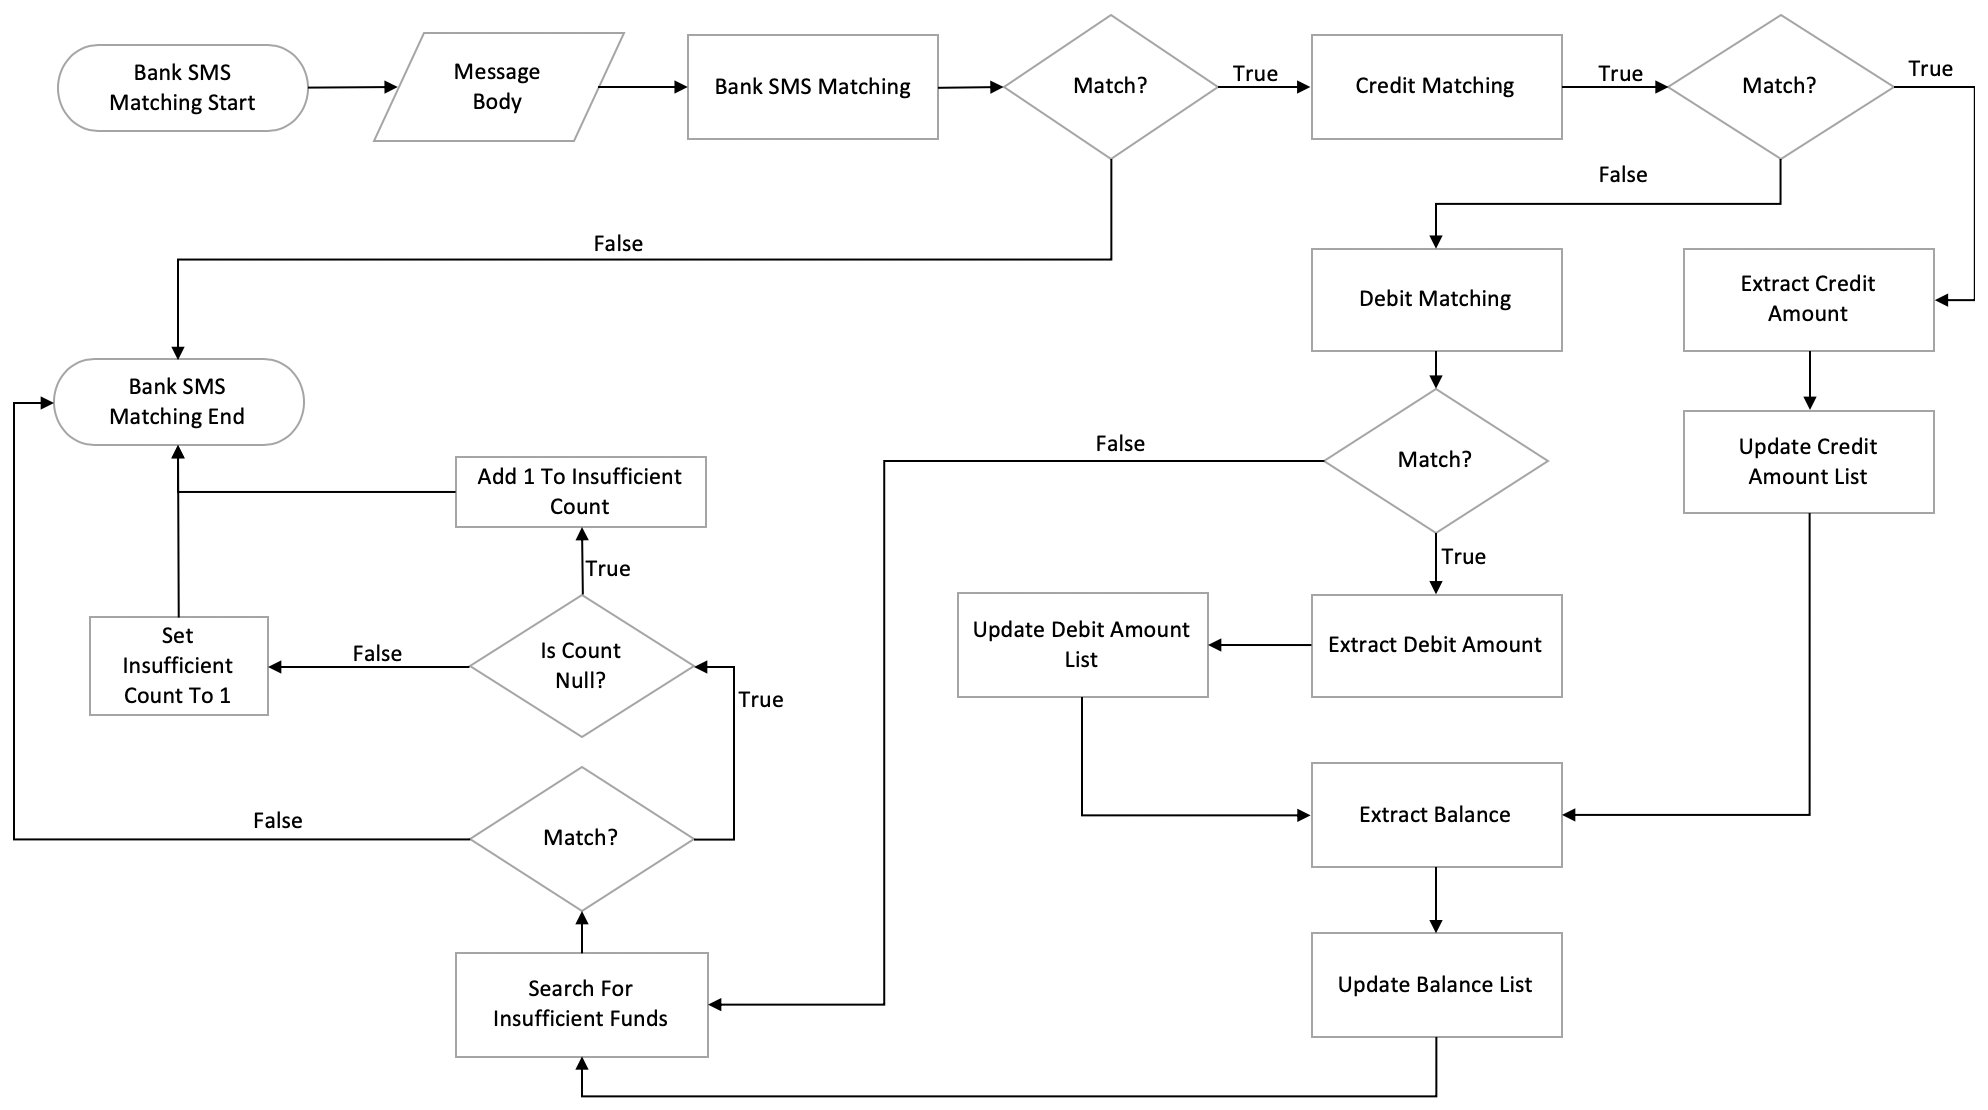
\includegraphics[width=0.95\textwidth]{images/bank_feats.png}
\caption{Bank Based Feature Generation}
\label{fig:bank_features}
\end{Figure}

\vspace{15pt}

\newpage

The competitor related features generated were:

\begin{itemize}
    \item The number of competitors that sent the client a message
    \item The number of competitors that sent a loan to the client
    \item The minimum and maximum loan amount received by, successful loan repayment made by, and unsuccessful loan repayment made by the client
    \item The number of loans received by, successful loan repayments made by, and unsuccessful loan repayments made by the client
    \item The number of rejected loan applications made by the client. 
\end{itemize}

\vspace{15pt}

The process of passing an SMS through the competitor related regular expressions and how features were generated throughout that process is represented in Figure \ref{fig:comp_features}. The process was completed for every SMS message received by a client within the 90 day period prior to their application. 

\vspace{15pt}

\begin{Figure}[!htb]
\centering
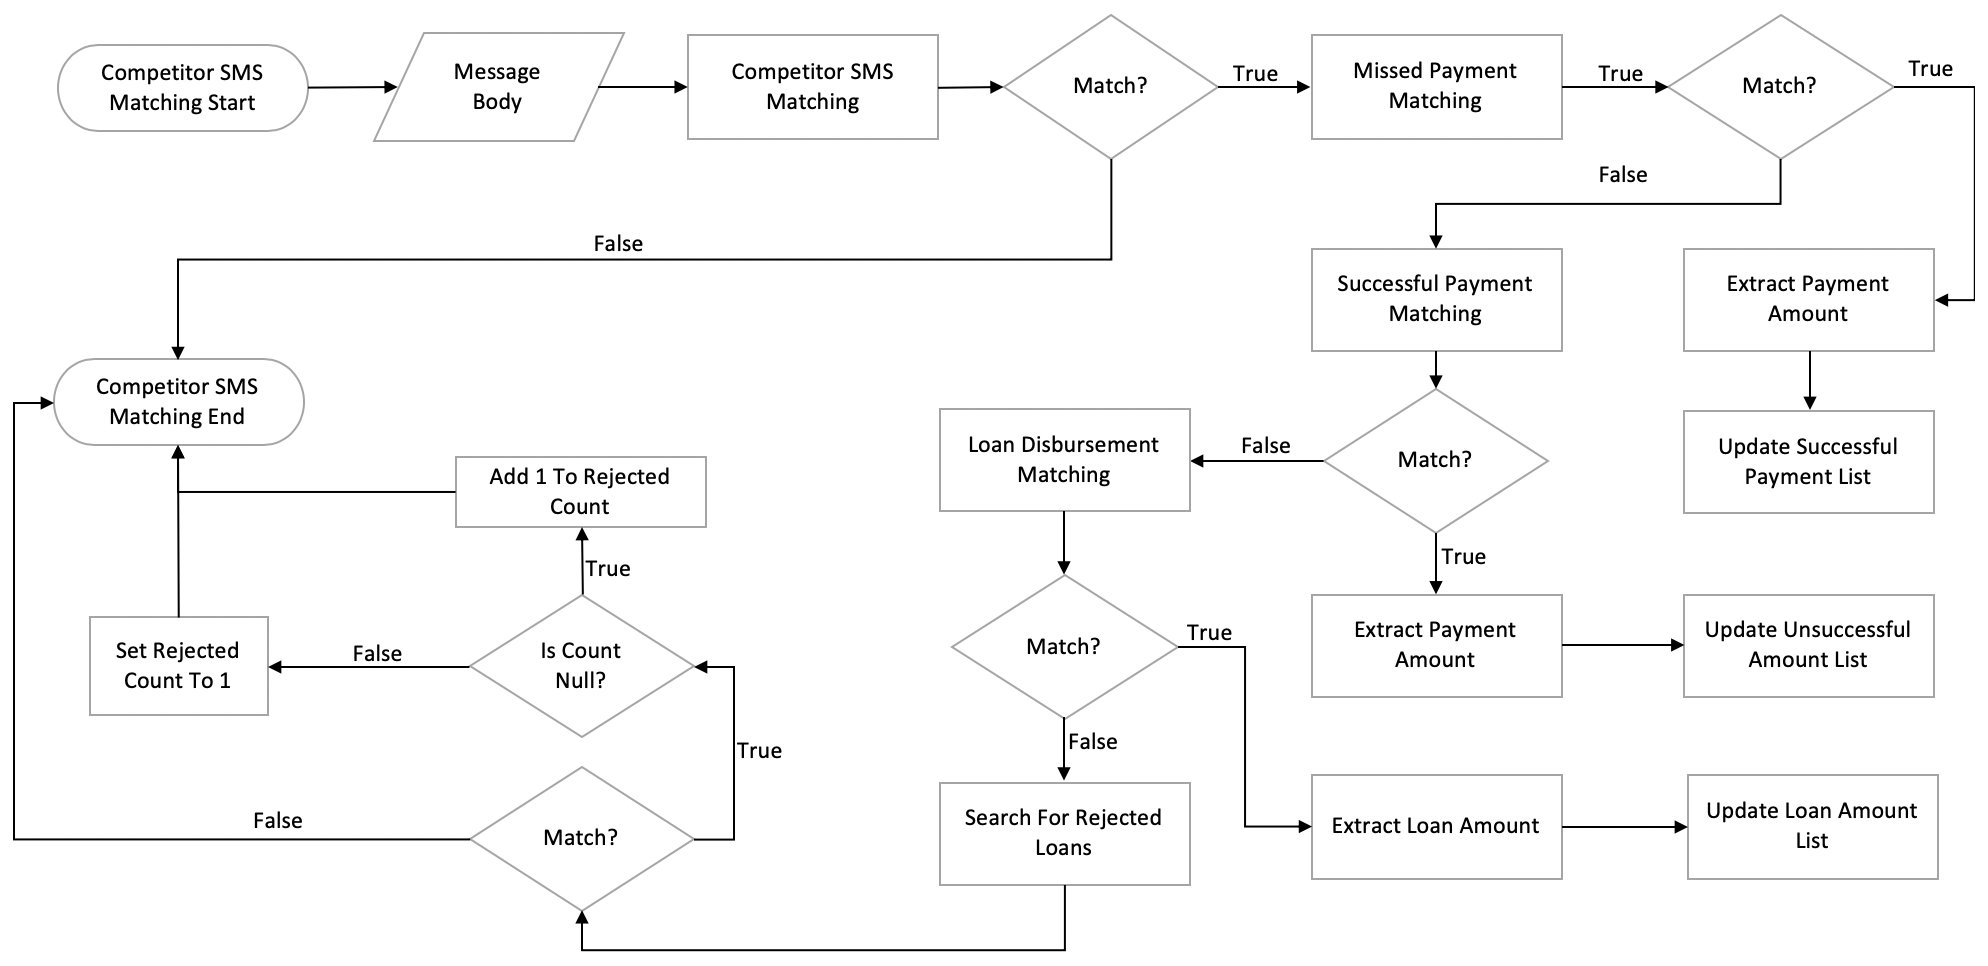
\includegraphics[width=0.95\textwidth]{images/comp_feats.png}
\caption{Competitor Based Feature Generation}
\label{fig:comp_features}
\end{Figure}

\vspace{15pt}


\subsubsection{Web Scraping}

The unique Android ID attached to each customer's cellular device, used to apply for their loan, was used to ascertain the brand and model of the device as well as the operating version currently used on the device. The brand of device and operating system system were used directly as features while the device brand name and model were used in conjunction to scrape the price of the device. \\

The script written to scrape and calculate the device price was written in Python and made use of the Beautiful Soup web scraping package. The price of each device was scraped from Jumia and Kara, two of the biggest Nigerian e-commerce platforms. The price was scraped from both websites by passing the name and model of the device into the respective search URL of each website. The Jumia search URL appears as follows \url{https://www.jumia.com.ng/phones-tablets/?q={NameAndBrand}&sort=Price}. \\

The logic used to derive a price for each customer's cellular device is shown in Figure \ref{fig:device}.

\vspace{15pt}

\begin{Figure}[!htb]
\centering
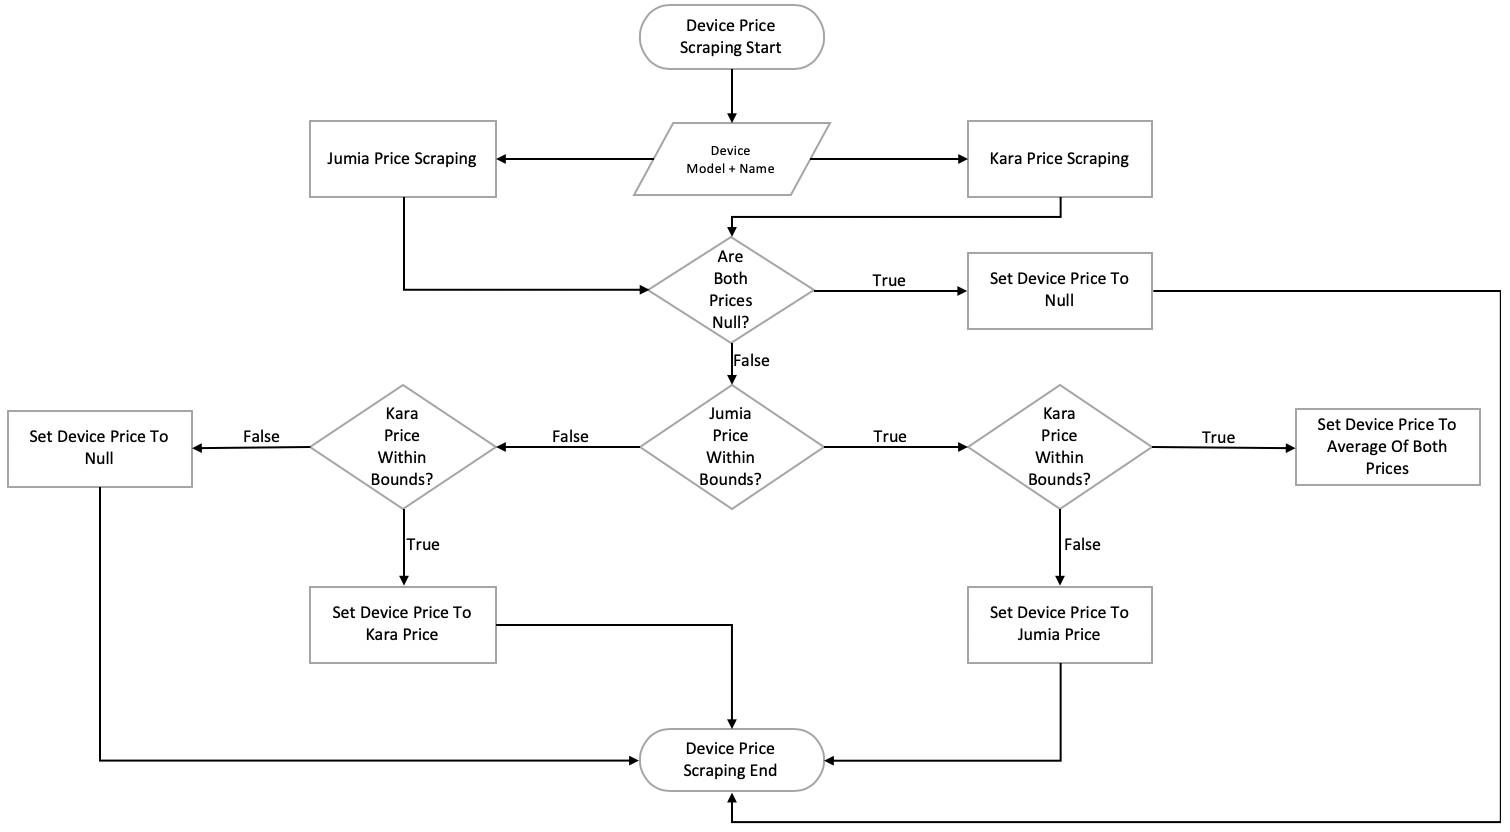
\includegraphics[width=0.9\textwidth]{images/device_price.png}
\caption{Device Price Logic}
\label{fig:device}
\end{Figure}

\vspace{15pt}



%---------------------------------------------------------------------------------------
%	SECTION 3
%---------------------------------------------------------------------------------------

\section{Preprocessing}

\subsection{Missing Values}


Matrix Decomp \\


\subsection{Categorical Variables}

Min Max Scaler

\subsection{Class Balancing}

Smote 
\chapter{Modelling Methods} 
\label{Chapter4}


\section{Parameter Tuning}

https://towardsdatascience.com/doing-xgboost-hyper-parameter-tuning-the-smart-way-part-1-of-2-f6d255a45dde

https://www.datacamp.com/community/tutorials/parameter-optimization-machine-learning-models

\section{Class Balancing}

Smote 

\section{Models}

\subsection{Logistic Regression}

\subsection{Random Forest}

\subsection{Extreme Gradient Boosting}

\subsection{Neural Network}

For the NN, no recurrent NN was used as they attempt to model time or sequence dependent behaviour. Which this case is not. 
\chapter{Results} 
\label{Chapter5}

tables and figures
\chapter{Conclusions and Recommendations} 
\label{Chapter6}

This chapter summarises the findings of the research aims of this masters dissertation displayed in Section 1.3. This chapter concludes by briefly describing the implications of the research conducted in this m.d. and the possible future research opportunities that could extend from the project.\\

\section{Research Questions}

The research aims of this project are are shown in Section 1.3, but for ease they are listed below:

\begin{itemize}
    \item Assess if augmenting sociodemographic and credit bureau data with the alternative features used in this project improves the overall performance of loan default prediction models.
    \item Determine if the alternative features used through this dissertation can be used to train accurate loan default prediction models. 
    \item Identify the optimal technique for developing loan default prediction models out of logistic regression, random forests, extreme gradient boosting, and a multi-perceptron neural networks. 
\end{itemize}

\vspace{10pt}

The first aim is answered by comparing the five holdout performance indicators of the models trained using the alternative features in conjunction with sociodemographic features, credit bureau features, and both the sociodemographic and credit bureau features against the performance indicators of the models trained using only sociodemographic, only credit bureau, and sociodemographic and credit bureau respectively for each of the 4 modelling techniques. \\

The performance indicators of the logistic regression, random forest, and XGBoost models developed using only sociodemographic or only credit bureau features improve when the datasets are augmented with alternative features. This trend is not seen in the performance indicators of the multi-layer perceptron models. However, for all 4 techniques used the best performing model uses all three data category combinations. Meaning, all models using sociodemographic and only credit bureau features improve when the datasets used to train them are augmented with alternative credit bureau features. \\

The second aim is addressed by assessing the performance indicators of all 4 models trained using only alternatives features. The indicators can be seen in the holdout results displayed in Chapter \ref{Chapter5}. The most accurate model trained using only alternative is an XGBoost model. The model has an overall accuracy of 0.68, a repaid accuracy of 0.78, an F1 score of 0.69, and an AUC measure of 0.63. These indicate that the model accurately predicts whether a loan will be repaid. However, the default accuracy of the model is 0.40. Meaning that the model does not accurately detect when a loan is likely to not be repaid. This is costly within the lending sector. \\

The third and final aim is assessed using a combination of model performance indicators and McNemar's Chi Squared test. The model performance indicators are used to infer the technique with the best performing indicators, while McNemar's Chi Squared test is used to determine if the models are significantly different. \\

The most suitable modelling technique - explored within this project - for loan default prediction is found to be XGBoost. This technique consistently produces the best performing model across all 7 data category combinations. The XGBoost models were proven to be significantly different from models of the other 3 techniques using McNemar's Chi Squared test. 


\section{Implications of This Research}

The research conducted throughout this projects answers the three research aims stated in Section 1.3. However, there are a number of ways in which the research into each of the aims could  strengthened. \\

The alternative features used throughout the project did not include the call log or contact data contained on each loan applicant's device. The research completed by \textcite{BigDataMicroFiance} showed that features developed from contact and call log data improved loan default prediction. Features similar to those used by \textcite{BigDataMicroFiance} could be added to the features used throughout this project  with the aim of further improving loan default prediction. \\

Only multi-layer perceptron neural networks were used throughout this project. \textcite{NNWest} displayed other NN architectures that were found to be suitable for loan default prediction. These NN architectures, as well as others, could be explored. \\

The hyper-parameters of every model trained and tested during this project are tuned using a grid-search. This method of parameter tuning requires manual input and does not necessarily lead to the most optimal models \parencite{NNWest}. The impact of Genetic algorithms - such as the one explored by \textcite{NNShen} - on loan default prediction performance could be explored. \\

Recursive feature elimination is the only feature selection method considered throughout this project. Furthermore, RFE is only used in conjunction with logistic regression to perform feature selection. Other selection methods and other base model types could be explored. \\  

Beyond how the res-arch methods used for this project could be strengthened, there are certain aspects of loan default prediction not explored by this m.d. Firstly, only first time loan applicants were considered for this project. The performance of each modelling technique on repeat lenders is not explored. \\

This project focuses on improving prediction in terms of overall accuracy, repaid accuracy, default accuracy, f1 score, and AUC. The financial implications of the loan default prediction models are not considered in the scope of the project. \\

The regulatory implications of the various data categories and modelling techniques used throughout this project are not explored. \\

Finally, the impact of improving loan default prediction on financial inclusion was not measured during this project. 


%----------------------------------------------------------------------------------------
%	BIBLIOGRAPHY
%----------------------------------------------------------------------------------------
\renewcommand{\baselinestretch}{1.5}
\printbibliography[heading=bibintoc]

%----------------------------------------------------------------------------------------


%----------------------------------------------------------------------------------------
%	THESIS CONTENT - APPENDICES
%----------------------------------------------------------------------------------------
\renewcommand{\baselinestretch}{1}

\appendix % Cue to tell LaTeX that the following "chapters" are Appendices

\chapter{Variable Definitions} % Main appendix title

\label{AppendixA} % Change X to a consecutive letter; for referencing this appendix elsewhere, use \ref{AppendixX}

Table \ref{table:variables} displays all variables used throughout this minor dissertation. The Table further displays a brief description of each variable, each variable's data type, and data category to which the feature belonged. 

\vspace{10pt}


\begin{longtable}{|p{2.5cm}|p{5.5cm}|p{2cm}|p{3.1cm}|}
\hline
\multicolumn{1}{|p{2.5cm}|}{Variable}&
\multicolumn{1}{|p{5.5cm}|}{Description}&
\multicolumn{1}{|p{2cm}|}{Data Type}&
\multicolumn{1}{|p{3.1cm}|}{Category}\\
\hline
Age & Age of applicant  & Numeric (Discrete) & Sociodemographic \\
\hline
App Count & Number of applications on th applicant's cellular device & Numeric (Discrete) & Alternative \\
\hline
Application Time & The time of day the loan application was made & Categorical & Alternative \\
\hline
Application Week & The week within the month the loan application was made  & Categorical & Alternative \\
\hline
Bank & The stated bank with which the applicant holds an account & Categorical & Sociodemographic \\
\hline
Banking Count & The number of financial applications on the clients cellular device & Numeric (Discrete)  & Alternative \\
\hline
Banks Contacted & The number of banks that sent an SMS messages to the applicant & Numeric (Discrete) & Alternative \\
\hline
Closed Accounts & The number of closed loan accounts the applicant has registered with the credit bureaus & Numeric (Discrete) & Credit Bureau \\
\hline
Competitor Count & The number of competing micro-finance companies that contacted the applicant & Numeric (Discrete) & Alternative \\
\hline 
Credit Transactions & The number of credit transactions extracted from SMS sent to the applicant from banks & Numeric (Discrete) & Alternative \\
\hline 
Debit Transactions & The number of debit transactions extracted from SMS sent to the applicant from banks & Numeric (Discrete) & Alternative \\
\hline 
Defaulted & A flag indicating whether or not a loan was repaid within 30 days of the repayment date & Numeric (Discrete) & Target \\
\hline 
Device Brand & The brand of the cellular device the applicant used to when applying foor their loan & Numeric (Discrete) & Alternative \\
\hline 
Device Price & The web-scraped price of the cellular device the applicant used when applying for their loan & Numeric (Discrete) & Alternative \\
\hline 
Employment Status & The employment status of the applicant & Categorical & Sociodemographic \\
\hline 
Gambling Count & The number of gambling applications on the applicant's cellular device & Numeric (Discrete) & Alternative \\
\hline 
Gender & The sex of the applicant & Categorical & Sociodemographic \\
\hline 
Highest Education & The highest level of education achieved by the applicant & Categorical & Sociodemographic \\
\hline 
Income & The stated monthly income of the applicant in Naira  & Numeric (Discrete) & Sociodemographic \\
\hline
Loan Purpose & The stated reason the applicant gave for applying for the loan & Categorical & Sociodemographic \\
\hline 
Lost Loans & The number of loan accounts deemed lost/unpaid the applicant has registered with the credit bureaus & Numeric (Discrete) & Credit Bureau \\
\hline 
Marital Status & The marital status of the applicant & Categorical & Sociodemographic \\
\hline 
Max Balance & The maximum balance extracted from the applicant's bank SMS & Numeric (Discrete) & Alternative \\
\hline 
Max Credit & The maximum credit transaction extracted from the applicant's bank SMS & Numeric (Discrete) & Alternative \\
\hline 
Max Debit & The maximum debit transaction extracted from the applicant's bank SMS & Numeric (Discrete) & Alternative \\
\hline 
Max Loan Amount & The maximum loan amount extracted from the SMS messages received by the applicant from other micro-finance companies & Numeric (Discrete) & Alternative \\
\hline 
Max Successful Loan Payment & The maximum successful loan repayment amount extracted from the SMS messages received by the applicant from other micro-finance companies & Numeric (Discrete) & Alternative \\
\hline 
Max Unsuccessful Loan Payment & The maximum unsuccessful loan repayment amount extracted from the SMS messages received by the applicant from other micro-finance companies & Numeric (Discrete) & Alternative \\
\hline 
Min Balance & The minimum balance extracted from the applicant's bank SMS messages & Numeric (Discrete) & Alternative \\
\hline 
Min Credit & The minimum credit transaction extracted from the applicant's bank SMS messages & Numeric (Discrete) & Alternative \\
\hline 
Min Debit & The minimum debit transaction extracted from the applicant's bank SMS messages & Numeric (Discrete) & Alternative \\
\hline 
Min Loan Amount & The minimum loan amount extracted from the SMS messages received by the applicant from other micro-finance companies & Numeric (Discrete) & Alternative \\
\hline 
Min Successful Loan Payment & The minimum successful loan repayment amount extracted from the SMS messages received by the applicant from other micro-finance companies & Numeric (Discrete) & Alternative \\
\hline 
Min Unsuccessful Loan Payment & The minimum unsuccessful loan repayment amount extracted from the SMS messages received by the applicant from other micro-finance companies & Numeric (Discrete) & Alternative \\
\hline 
Missed Payments & The number of instalments missed by the applicant on their loans registered with the credit bureaus & Numeric (Discrete) & Credit Bureau \\
\hline 
News Count & The number of news related applications cellular device & Numeric (Discrete) & Alternative \\
\hline 
Non-performing Loans & The number of active loans where the applicant has missed an instalment and the loan was registered with the credit bureaus & Numeric (Discrete) & Credit Bureau \\
\hline 
Num Applications& The number of rejected applications the applicant had with the micro-finance company prior to their applicant under consideration & Numeric (Discrete) & Sociodemographic \\
\hline 
Num Applications& The number of rejected applications the applicant had with the micro-finance company prior to their applicant under consideration & Numeric (Discrete) & Sociodemographic \\
\hline 
Paid Loans & The number of fully repaid loans the applicant has registered with the credit bureaus & Numeric (Discrete) & Credit Bureau \\
\hline 
Performing Loans & The number of active loans where the applicant has not missed an instalment and loan was registered with the credit bureaus & Numeric (Discrete) & Credit Bureau \\
\hline 
Property Status & The current ownership status of the property where the applicant resides & Categorical  & Sociodemographic \\
\hline
Rejected Loans & The number of rejected loan applications extracted from the SMS messages received by the applicant from other micro-finance companies & Numeric (Discrete) & Alternative\\
\hline 
Sector & The sector the applicant's occupation falls under & Categorical & Sociodemographic \\
\hline 
State & The Nigerian state in which the applicant resides & Categorical & Sociodemographic \\
\hline 
Successful Payments & The number of successful loan repayments extracted from the SMS messages received by the applicant from other micro-finance companies & Numeric (Discrete) & Alternative \\
\hline 
Time at Current Address & The time in months the client has spent at their current residence & Numeric (Discrete) & Sociodemographic \\
\hline 
Time at Employer & The time in months the client has spent at their current employer & Numeric (Discrete) & Sociodemographic \\
\hline 
Unsuccessful Payments &  The number of unsuccessful loan repayments extracted from the SMS messages received by the applicant from other micro-finance companies & Numeric (Discrete) & Alternative \\
\hline 
VPN Count &  The number of virtual private network applications on the applicant's cellular device & Numeric (Discrete) & Alternative \\
\hline 
\caption{Variables Used in Models}
\label{table:variables}
\end{longtable}


\vspace{10pt}

\end{document}  
